% Self-contained section; requires amsmath.
\section{A larger lower bound}
Write $V$ for the volume of any universal body $K$. Three witnesses force
a unit segment in $K$, a planar curve of planar width greater than
$b=0.43892$, and a space curve of width greater than $w=0.25607$.
These are respectively the segment, the rescaled Adhikari--Pitman caliper,
and the rescaled Bartels--Choy--Wu--Li curve as in the original report.
A fourth witness forces a ball. For the strongest endpoint below, take $r=1/9.577$. Zalgaller's open inspection curve has length to hull-inradius ratio below $9.577$ \cite[p.~125, following Theorem~1.2]{ghomi}. Enclosing the curve encloses its convex hull. An independent rational polygon in the accompanying code gives $r=0.1043499$ and a lower bound within $0.000005$ of the stronger one. The two widths follow from the respective width-one lengths $<2.27830$ and $<3.90513$ \cite{ap,bartels}. Each witness is free to occupy its own position.

Project $K$ perpendicular to its unit segment, onto a planar body $P$
of area $A$, perimeter $p$, and diameter $d$. We have $d\ge b$ and
every width of $P$ is at least $w$. Indeed the plane of the caliper contains
some direction parallel to the projection plane, and the spatial width
bound holds in all directions. To see $3V\ge A$, observe that fibers parallel to the
unit segment have length at least $t$ on a $(1-t)$-scaled copy of $P$,
by taking convex combinations with the segment. Integrating their superlevel areas gives $V\ge A\int_0^1(1-t)^2\,dt=A/3$.

Let $S$ denote the surface area of $K$ and $m$ its unit outer normal,
defined almost everywhere. Write $m_u,m_H$ for its component along
the unit segment and its horizontal projection. The projection area
formula gives $\int|m_u|\,dS=2A$. For a horizontal unit normal $e$, the
projection of $K$ onto $e^\perp$ contains the unit segment and has transverse
span $W_P(v)$, where $v$ is the horizontal unit vector perpendicular to $e$.
Taking the two triangles on the segment gives projected area at least
$W_P(v)/2$. Integrate over $e$ on the horizontal unit circle.
The projection formula and $\int|m_H\cdot e|\,de=4|m_H|$ give
$2\int|m_H|\,dS\ge p$, using $\int W_P(v)\,dv=2p$.
The triangle inequality for integrals now gives
$S\ge\sqrt{(p/2)^2+(2A)^2}$. Since $K$ contains an $r$-ball,
the divergence theorem about its center gives $3V\ge rS$
(equivalently, sum the volumes of the pyramids over the facets and
take a polyhedral limit).


Choose a diameter of $P$ as base from $O=(0,0)$ to $B=(d,0)$. Every point has first coordinate in $[0,d]$. Take a highest and a lowest point $C=(x,h)$ and $F=(y,-k)$ and let $H=h+k$. The quadrilateral $Q=\operatorname{conv}\{O,B,C,F\}$ has area $dH/2$. Thus $2A\ge dH\ge bw$. The perimeter $p$ bounds the length of the quadrilateral's two broken paths $OCB$ and $OFB$. By reflecting across each horizontal extremal line, their lengths are at least $\sqrt{d^2+4h^2}$ and $\sqrt{d^2+4k^2}$, respectively.
\begin{center}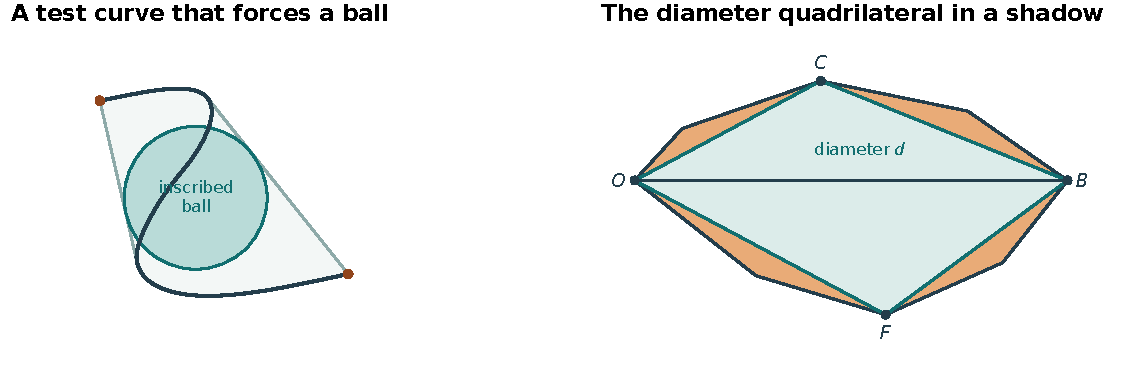
\includegraphics[width=.92\linewidth]{figures/lower_geometry.pdf}\end{center}
{\small\sffamily\color{ink}Left, the independent 61-vertex test curve and the orthogonal shadow of its inscribed ball. Right, the excess area is the sum of the four orange regions between the shadow boundary and the quadrilateral.}
\paragraph{How the two oblique widths use the excess area.}
Retain the notation $A,d,H,h,k,x,y$ of the diameter quadrilateral.
Reflect vertically if necessary so that $0\le h\le k$ and write $f=h/H$.
Set $E=A-dH/2$. The surface and the two reflected polygonal paths imply
\begin{equation}
 (3V)^2\ \ge\ r^2\left[
 \tfrac14\left(\sqrt{d^2+4H^2 f^2}
       +\sqrt{d^2+4H^2(1-f)^2}\right)^2+d^2H^2\right].
 \label{eq:edge-surface}
\end{equation}
In fact $S\ge\sqrt{(p/2)^2+(2A)^2}$, $3V\ge rS$, and $2A\ge dH$.

For the upper supporting vertex $C=(x,h)$, define $e_{ul}$ and $e_{ur}$
as the areas of the portions of $P$ beyond the lines $OC$ and $CB$,
on the side away from triangle $OCB$. Define $e_{bl},e_{br}$ in the
reflected lower half analogously, using $F=(y,-k)$. These four portions
have disjoint interiors and total area $E$. Indeed, on the upper half the
two outside tests have left sides
\[
  U=xY-hX,\qquad T=h(X-x)+(d-x)(Y-h)
\]
at a point $(X,Y)$. Their sum is $d(Y-h)\le0$, and neither is positive on
the lower half. If $T>0$, the triangle with the point and the edge $CB$
lies in the upper-right portion, so $T\le2e_{ur}$. The same argument
gives $U\le2e_{ul}$, with corresponding formulas below.

Assume first $h>0$ and take
\[
 a_+=\max\{(d-x)/h,\ y/k\},\qquad
 a_-=\max\{x/h,\ (d-y)/k\}.
\]
The maximum of $X+a_+Y$ exceeds $x+a_+h$ by at most $2e_{ur}/h$.
This follows from
\[
   X-x+a_+(Y-h)=T/h+\bigl(a_+-(d-x)/h\bigr)(Y-h).
\]
Its minimum is at least $y-a_+k-2e_{bl}/k$ by the reflected
lower-left inequality. Its width is at least $w\sqrt{1+a_+^2}$. Applying
the same argument to $-X+a_-Y$ uses the two remaining edge areas.
On addition the horizontal offsets $x-y$ cancel, giving, with
$s=a_++a_-$,
\[
   w\sqrt{4+s^2}\ \le\ w\bigl(\sqrt{1+a_+^2}+\sqrt{1+a_-^2}\bigr)
    \ \le\ Hs+2E/h .
\]

Here $k\ge h$. For $D_*=hs$, the last inequality becomes
\[
 w(\sqrt{D_*^2+4h^2}-D_*)\le 2A-dw+(H-w)(D_*-d).
\]
The left side decreases with $D_*$, while the right side increases. Upper bounds on $D_*$ will suffice.

Put $t=h/k$, $X_0=|x-d/2|$ and $Y_0=|y-d/2|$. Expand the two maxima defining $s$. After multiplying by $h$, their possible sums are $d$, $dt$, $x+ty$, and $(d-x)+t(d-y)$. Consequently
\[
 d\le D_*\le d+\Delta,\qquad
 \Delta=\min\{dt,\max(0,-d(1-t)/2+X_0+tY_0)\}.
\]
Suppose now that $3V\le A_0$. The surface inequality gives $p\le p_{\max}=2\sqrt{(A_0/r)^2-d^2H^2}$. The upper broken path $OCB$ has length at most $\ell=p_{\max}-\sqrt{d^2+4k^2}$. Thus $C$ belongs to the ellipse of foci $O,B$ and major axis $\ell$. From its equation,
\[
 X_0\le\min\left\{d/2,\frac{\ell}{2}\sqrt{1-\frac{4h^2}{\ell^2-d^2}}\right\}.
\]
The case $\ell<\sqrt{d^2+4h^2}$ immediately contradicts the upper path's length. Interchanging $h,k$ bounds $Y_0$ as well. If $h=0$, the perimeter test alone applies.

\paragraph{The finite check.}
For $A_0=3(0.018975)$, the only possible parameter box is
\[
 b\le d\le2A_0/w,\quad w\le H\le2A_0/b,\quad 0\le f=h/H\le1/2.
\]
The included checker bisects it into 24 boxes. In each box the sum of the two square roots in \eqref{eq:edge-surface} is bounded below using the lower endpoints for $d,H$ and the upper endpoint for $f$, since that sum decreases as $f$ increases to $1/2$. The area bound $dH\le2A_0$ tightens both upper endpoints. For each ellipse, an upper bound on $\ell$ and lower bounds on its own height and the focal distance give upper bounds on the two offsets. The checker substitutes an upper bound for $D_*$ and a lower bound for $h$ in the decreasing left side of the oblique-width test, and upper bounds for $A,H,\Delta$ and a lower bound for $d$ on its right. When a box still overlaps $h=0$, the offset bound $d/2$ suffices. In the zero-height case the oblique-width test reduces to $0\le2A-dw$, so a width exclusion cannot accidentally discard a feasible zero-height case.
All arithmetic is rational with outward rounding of square roots at precision $10^{-12}$. Seventeen boxes fail the surface or ellipse test and seven fail the width test. This proves $V>0.018975$.

Using the explicit polygon in \texttt{check\_inspection.py} gives $V>0.01897$ by the identical 23-bisection calculation with $r=0.1043499$. Its 61 vertices are integer triples in units of $10^{-7}$. Rounding each integer link length upwards bounds the path length by $0.9999834$. Every facet plane contains a noncollinear triple. The checker enumerates all triples and tests every supporting plane $n\cdot X=c$ in integer coordinates, oriented outwards. It finds $c>0$ and $c^2\ge(1043499)^2\|n\|^2$ for every supporting triple, proving ball containment.
